\newcommand{\real}{\mathbb{R}}
\newcommand{\nnatural}{\mathbb{N}}
\newcommand{\cE}{\mathcal{E}}
\newcommand{\cF}{\mathcal{F}}
\newcommand{\cI}{\mathcal{I}}
\newcommand{\cM}{{\mathcal{M}}}
\newcommand{\cN}{{\mathcal{N}}}
\newcommand{\cIMN}{\mathcal{I}_{\mathcal{N}, \mathcal{M}}}
\newcommand{\Fix}{\mathit{Fix}}
\newcommand{\stirlingii}{\genfrac{\{}{\}}{0pt}{}}

\documentclass{beamer} 
%\documentclass[a4paper, 11pt, xcolor=dvipsnames]{beamer} 
\usepackage[polish]{babel}
\usepackage[utf8]{inputenc}
\usepackage{t1enc}
\usepackage{amsmath}
\usepackage{graphics} 
\usepackage{fancybox} 
\usepackage{makecell}

%\usepackage{helvet}
%All font families are not available in every Beamer installation, but
%typically, at least some of the following families will be available:
%    serif          avant        bookman      chancery        charter
%     euler         helvet       mathtime       mathptm       mathptmx
%    newcent      palatino        pifont        utopia

\mode<presentation> {
\usetheme{Madrid} 
}
\usepackage{graphicx} % Allows including images
\usepackage{booktabs} % Allows the use of \toprule, \midrule and \bottomrule in tables

%%% to co nizej to byl standardowy temat:
%\usecolortheme[rgb={0.1,0.6,0.3}]{structure}
%%% na razie taki :-)
\usecolortheme[named=violet]{structure}
%\usecolortheme[named=RubineRed]{structure} 
%\usecolortheme[named=CarnationPink]{structure}
\begin{document} 
%\setbeamercovered{transparent=15} %Ukryte (np przez uncover beda polwidoczne)
\setbeamercovered{dynamic}        %Ukryte (np przez uncover beda polwidoczne, im blizej tym mocniej)
%%% to ponizej tez nie dziala...
%\transglitter[direction=90]
%%% to nizej mialo zmienic kolor bibliografii lecz niestety nie zadzialalo.
%\setbeamercolor{bibliography item}{fg=black}
%\setbeamercolor*{bibliography entry title}{fg=black}
%-----------------------------------
\title[Kwadraty łacińskie]{
  Kwadraty łacińskie i zagadnienia pokrewne.
} 
%\subtitle{}
\author{} 
\date{\today}
%---------------------
\begin{frame} 
  \titlepage 
\end{frame} 
%---------------------
%\section[Outline of the talk]{}
%\frame{\tableofcontents}
%----------------------------------
%\section{Introduction}
\begin{frame}
\uncover<1->{
\begin{block}{Prostokąt łaciński}
  To macierz która posiada elementy parami różne
  we wszystkich wierszach i kolumnach.
  Jeśli prostokąt łaciński jest macierzą
kwadratową to nazywamy ją {\bf Kwadratem łacińskim}
\end{block}
}
\uncover<2->{
\begin{block}{The latin rectangles}
  
  A matrix such that has pairwise different
  elements in each column and in each row.
  If the latin rectangle is a square matrix
  then we call it {\bf a latin square}.
  
\end{block}
}
\uncover<3->{
  We usually assume that we build a latin square
  of size $n \times n$ with an elements
  from the set $\lbrace 1, \ldots , n\rbrace$
  {\bf or better }, \underline{a latin}
  letters $a, b, \ldots $.
}
\end{frame}

\begin{frame}
  Examples:
  $\begin{bmatrix}
    a & b & c & d\\
    b & d & a & c\\
    d & c & b & a\\
    c & a & d & b\\
    \end{bmatrix}$


\end{frame}

\begin{frame}
  \uncover<1->{
  \begin{block}{Theorem}:
    Each $n \times m$ latin rectangle ($n < m$) can be
    completed to a $(n + 1) \times m$ latin rectangle.
  \end{block}
  }
  {\bf Proof:} Use the Hall's theorem.
  \uncover<2->{
    \begin{block}{Corollary}
      Each $n \times m$ latin rectangle ($n < m$)
      can be completed to a full latin square.
      \end{block}
  }
  \end{frame}

\begin{frame}
  \begin{block}{Kwadraty {\bf grecko-łacińskie (Graeco-Latin squares)}
      (zwane też {\bf kwadratami Eulera}
      - historia (called also the {\bf Euler squares} - the history of them in a nutshell}
  \end{block}

  \begin{itemize}
  \item<1->
    {\color{blue} Problem 36 oficerów (36 officers problem)}:
    L.Euler [1782]: Nie istnieje kwadrat grecko-łaciński $6\times 6$
      (There is no a Graeco-Latin square of size $6 \times 6$).
  \item<2->G.Tarry [1900] Potwierdzona (Verified (of course, without computer
    support 
\includegraphics[height=3mm]{smile.png})).
  \item<3-> Euler sądził że istnieje kwadrat grecko-łaciński wtedy
    i tylko wtedy gdy $n - 2$ jest podzielne przez $4$.

    Euler speculated that Graeco-Latin squares exists if and
    only if $n \equiv 2 (\pmod 4)$.
  \item<4-> R.C.Bose, S. S. Shrikhande, E.T.Parker [1960]:
    Dla wszystkich $n$ poza $2$ i $6$ istnieje kwadrat
    grecko-łaciński.( For each $n \not= 2,6$ there exists a
    Graeco-Latin square.)
    \end{itemize}
\end{frame}

\begin{frame}
\begin{center}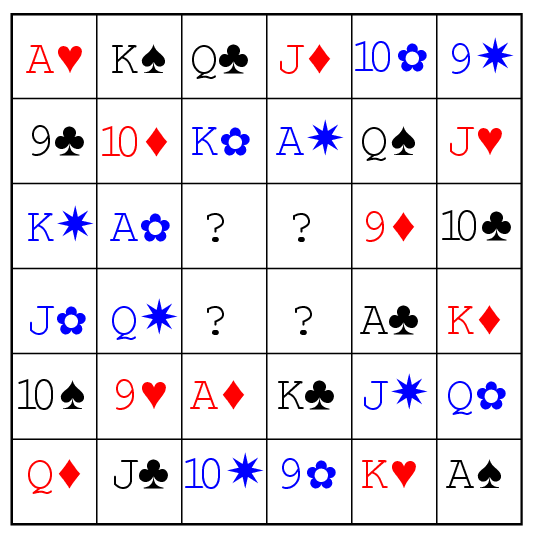
\includegraphics{36_oficerow.png}\end{center}
  
  \end{frame}

\end{document}

